%!TEX root = ../../report.tex
\section{Dynamic map on the MiR-100}

The system is built to be run with the MIR100 robot. This involves constructing and interfacing the dynamic map system with the Robot Operating System (ROS) used by the robot. In figure \ref{fig:mir_interface} is shown the developed system along with the existing nodes that interacts with it. 

\begin{figure}[htbp]
	\centering
	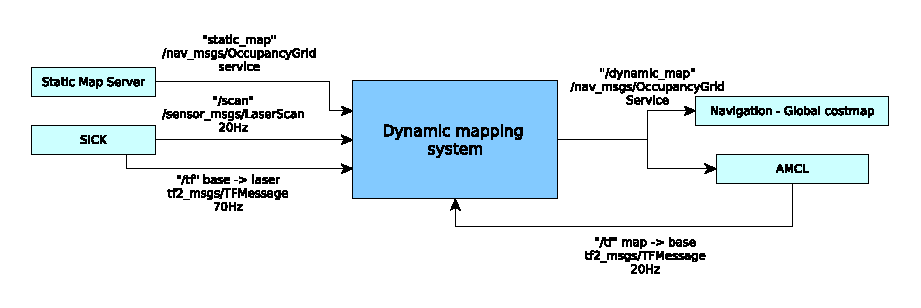
\includegraphics[width=1\linewidth]{chapters/cost_interpretation/figures/dynamic_map_mir_interface.eps}
	\caption{The Dynamic Map Server with connected nodes and interface}
	\label{fig:mir_interface}
\end{figure}

The dynamic map server receives a static map from the static map server in order to initialize the dynamic learner. This is only done at startup. The primary input for the dynamic map server is the laser scan data provided by the SICK node and the position of the scanners in the world, provided by the SICK and AMCL nodes in conjunction. The position of the scanners on the robot is provided by the SICK system and the robot position in the world is published by AMCL. 
The Dynamic Map Server is based on the ROS of Layered costmap \cite{lu2014layered}. Each layer in the layered costmap maintains its own costmap and these are combined to produce the final costmap. Figure \ref{fig:dynamic_map_server_internal} shows the elements of the Dynamic Map Server and their dataflow. The layered costmap in the Dynamic Map Server contains two layers: The Activity Layer and the Blueprint Layer. 

\begin{figure}[htbp]
	\centering
	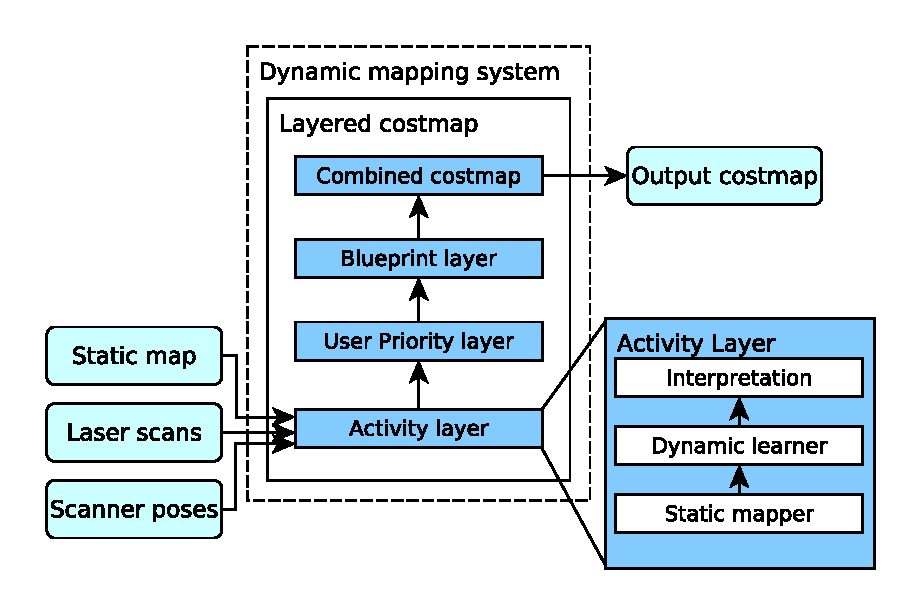
\includegraphics[scale=0.7]{chapters/cost_interpretation/figures/implementation_overview.eps}
	\caption{The Dynamic Map Server internal components}
	\label{fig:dynamic_map_server_internal}
\end{figure}

The Activity Layer is the primary layer and handles the mapping, learning of the dynamics and interpretation of the dynamics. It delivers a costmap that should contain the learned static obstacles with a high cost and dynamic obstacles with a cost appropriate to its dynamic. The second layer that is currently available in the Dynamic Map Server is the Blueprint Layer. This layer is designed to specify minimum costs associated with a cell. This could be used to ensure that certain areas would be avoided or avoid any possible erosion, of the walls in the map representation, due to erroneous localization. Because the Dynamic Map Server is implemented as a layered costmap it is possible add new layers to it for specific use-cases by means of a simple ROS API.